\documentclass{article}

\usepackage[utf8]{inputenc}   %for german letters ä,ö...
\usepackage[ngerman]{babel}   %german settings
\usepackage{amsmath}
\usepackage{amssymb}
\usepackage{tikz}
\usepackage{caption}
\usepackage[left=3cm,right=3cm,top=2cm,bottom=3cm]{geometry}
\usepackage{siunitx}
\usepackage{esdiff}
\usepackage{braket}
\usepackage{subcaption}
\usepackage{booktabs}
\usepackage[outdir=./]{epstopdf}
\usepackage{lscape}

\sisetup{locale = DE}

\newcommand{\RM}[1]{\MakeUppercase{\romannumeral #1}}

\usepackage[backend=bibtex8,sorting=none]{biblatex}
\addbibresource{refs.bib}

\usetikzlibrary{arrows,snakes,shapes}
\usetikzlibrary{trees}
\usetikzlibrary{decorations.pathmorphing}
\usetikzlibrary{decorations.markings}

\newcommand{\upd}[1]{^\mathrm{#1}}
\newcommand{\ind}[1]{_\mathrm{#1}}

\begin{document}
\setlength{\parindent}{0em}   %Einrücken verhindern
\title{Physikalisches Praktikum \RM{4}\\Versuch 428\\Röntgenstrahlung und Materialanalyse}
\author{Friedrich Hübner \qquad s6frhueb@uni-bonn.de \qquad 2897111\\
  Kilian Bönisch \ \ \ \qquad s6kiboen@uni-bonn.de \qquad 2897138}
\date{11.12.17 und 12.12.17}

\maketitle

\thispagestyle{empty}

\newpage

Bereits Anfang des 20. Jahrhunderts wurde die Höhenstrahlung entdeckt. Trotzdem kennt man weitgehend auch heute noch nicht ihre Ursachen. Mittlerweile wird mit großem Aufwand versucht, der Herkunft der Höhenstrahlung auf die Spur zu kommen. Ein wichtiger Aspekt ist dabei die Beobachtung der sekundären kosmischen Strahlung, welche durch die Wechselwirkung der ursprünglichen Strahlung mit der Atmosphäre entsteht. In diesem Versuch wird im ersten Teil die Winkelverteilung der Teilchen aus der sekundären Höhenstrahlung vermessen. Im zweiten Versuchsteil wird außerdem die Verteilung der Zerfallszeiten der kosmischen Myonen bestimmt.   


\section{Theoretische Grundlagen}

\subsection{Tunneleffekt}
Bei der Rastertunnelmikroskopie tastet eine leitende Sonde mit dünner Spitze eine Probe ab. Das Vakuum (bzw. die Luft) zwischen Spitze und Probe stellt für Elektronen aus der Spitze eine Potentialbarriere dar, da sie sich in der Spitze in einem gebundenen Zustand befinden. Klassisch könnte kein strom zwischen Spitze und Probe fließen wenn die gebundenen Elektronen eine Energie $E$ kleiner als die Potentialbarriere haben. Quantenmechanisch kann durch den Tunneleffekt jedoch ein Strom fließen. Um diesen Effekt zu verstehen wird die Potentialbarriere stark vereinfacht als ein Kastenpotential mit Höhe $V$ betrachtet. Außerdem wird angenommen, dass die Elektronen in Spitze und Probe als frei betrachtet werden können. Die stationären Zustände der resultierenden Schrödingergleichung können nun leicht berechnet werden. Der Transmissionswahrscheinlichkeit $T$ für eine von der Spitze zur Probe laufende Materiewelle ist dann gegeben durch
\begin{align*}
  \frac{1}{T}=1+\frac{1}{4}\left( 2+\frac{E}{V-E} + \frac{V-E}{E}\right) \sinh^2\left( 2a \frac{\sqrt{2m(V-E)}}{\hbar} \right), 
\end{align*}
wobei $m$ die Elektronenmasse und $a$ die Ausdehnung des Potentials ist.
Für große $Va$ gilt also
\begin{align*}
  T \propto e^{-4a\sqrt{2m(V-E)}/\hbar}. 
\end{align*}  
Der Tunnelstrom hängt also stark von dem Abstand $a$ ab. Genau diese starke Abhängigkeit wird bei der Rastertunnelmikroskopie ausgenutzt. 


\subsection{Balmer-Serie}
Die Energie-Eigenzustände des Wasserstoffatoms werden durch die Quantenzahlen $n,l$ und $m$ beschrieben. Ein Zustand mit der Hauptquantenzahl $n$ hat dabei den Energie-Eigenwert $E_n=-Ry/n^2$, wobei $Ry$ die Rydberg-Energie ist. Wechselt das Wasserstoffatom von einem Zustand mit Hauptquantenzahl $n$ zu einem energetisch niedrigeren Zustand mit Hauptquantenzahl $n'$ wird ein Photon der Energie 
\begin{align}
  E_{n \rightarrow n'}=Ry \left( \frac{1}{n'^2} - \frac{1}{n^2}\right)
\end{align}
emittiert. Die Balmer-Serie enthält alle Frequenzen des Emissionsspektrums, die aus dem Übergang von einem Niveau $n>2$ auf das Niveau $n'=2$ entstehen.

\subsection{Linienbreite}
In der Praxis werden die mit dem Reflexionsgitter beobachtbaren Balmer-Linien eine gewisse Ausdehnung haben, mögliche Ursachen dafür sind:
\begin{itemize}
\item
Im Versuch wird das Spektrum von einem Gemisch aus Deuterium und normalem Wasser in einer Gasentladungsröhre untersucht. Durch die abweichende reduzierte Masse von Deuterium und Wasserstoff ändert sich auch das Emissionsspektrum leicht, so, dass es zu einer Aufspaltung der Linien kommt, der Isotopieaufspaltung.
\item    
Durch die thermische Bewegung der Atome kommt es zur Dopplerverschiebung der Wellenlänge des emittierten Lichtes. Bewegt sich das Atom mit der Geschwindigkeit $v$ auf den Empfänger zu und emittiert ein Photon der Wellenlänge $\lambda$, so misst dieser die Wellenlänge 
\begin{align*}
  \lambda'=\lambda \cdot \left(  1+ \frac{v}{c} \right),
\end{align*} 
wobei $c$ die Lichtgeschwindigkeit ist. Nimmt man an, dass es sich bei dem Gas der Gasentladungsröhre um ein ideales Gas handelt gilt für die Geschwindigkeit $v$ jedes Atoms (mit Masse $m$ und Boltzmann-Konstante $k_\mathrm{B}$)
\begin{align*}
  \frac{1}{2} m v^2=\frac{3}{2} k_\mathrm{B} T.
\end{align*}
Durch die Dopplerverschiebung schwankt die Wellenlänge also im Bereich
\begin{align}
  \lambda'=\lambda\left(1 \pm \frac{1}{c}\sqrt{\frac{3k_\mathrm{B}T}{m}} \right).
\end{align}
\item
Nach \cite{unschaerfe} gilt, dass wenn ein angeregter Zustand des Atoms die mittlere Lebensdauer $\tau$ hat, die Spektrallinie dieses Zustandes die Form einer Lorentz-Kurve mit Breite 
\begin{align}
  \Delta E=\frac{\hbar}{\tau}
\end{align}
hat.
\end{itemize}


\subsection{Durchführung}
Für den Franck-Hertz-Versuch wird zunächst der Ofen auf eine Temperatur von etwa $165^\circ$C geheizt. Mit dem Computer werden die Spannung $U_\mathrm{A}$ (proportional zu $I_\mathrm{A}$) und die Beschleunigungsspannung $U_\mathrm{B}$ aufgenommen. Der Aufbau erlaubt ein automatisches Hochfahren der Beschleunigunsspannung bis zu einem eingestellten Maximalwert. Bei der eingestellten Temperatur von $T=165^\circ$C wird für vier verschiedene Gegenspannungen die Kennlinie aufgenommen. Anschließend wird die Kennlinie bei fester Gegenspannung für vier verschiedene Temperaturen aufgenommen.

\subsection{Winkelverteilung}
\subsubsection{Schwellenkurve}
Bevor man die Winkelverteilung messen kann, muss zuerst die optimale Schwelle für den Diskriminator D12 bestimmt werden. Dazu wird die Schwelle des Diskrimators von -50 bis -250 \si{\milli\volt} in 10 \si{\milli\volt} Schritten verändert und jeweils für 2520 \si{\second} die Anzahl der Koinzidenzen von D12 mit D23, D24, D1 oder D2 gemessen. Dies wird über ein LabVIEW-Programm automatisiert (siehe Abb. \ref{fig:prog_all}).\\

\begin{figure}
\centering
\includegraphics[height=20cm]{data/friedrich/prog_ges_rot.png}
\caption{Gesamtes Programm}
\label{fig:prog_all}
\end{figure}

Im ersten Teil des Programmes wird die Hardware initialisiert (siehe Abb. \ref{fig:prog_init}). Im wesentlichen werden die Diskrimatoren D12 (Id 3), D23, D24, D1, D2 (Ids 1, 4, 5, 7) und D25 (Id 7) mit einer LED verbunden. Danach wird das ODER-Signal aus den Signalen D23, D24, D1 und D2 ermittelt, indem man sie über Oder-Blöcke verknüpft. Das Ausgangssignal wird wieder auf eine LED gegeben. Um Signale zu zählen werden Koinzidenzzähler verwendet. Zähler 1 zählt Koinzidenzen aus D12 und dem ODER-Signal, Zähler 2 die Anzahl der Signale in D12, Zähler 3 die ODER-Signale und Zähler 4 die Signale aus D25. \\
 
\begin{figure}
\centering
\includegraphics[height=20cm]{data/friedrich/prog_init.png}
\caption{Hardwareinitialisierung}
\label{fig:prog_init}
\end{figure}

Der zweite Teil besteht aus zwei verschachtelten Schleifen (siehe Abb. \ref{fig:prog_prog}). Vor der äußeren Schleife wird die Schwelle auf einen Startwert gesetzt (-50\si{\milli\volt}) und fünf Arrays initialisiert (eines, um die Schwellenwerte zu speichern und die anderen vier für die Anzahl der Ereignisse in den Koinzidenzzählern). Die äußere Schleife setzt den Schwellenwert des Diskriminators und speichert ihn im Array, wartet dann 2520\si{\second} und fügt dann die gemessenen Koinzidenzen der einzelnen Koinzidenzzähler an die jeweiligen Arrays ein. Danach werden die Zähler zurückgesetzt und die Schwelle um 10 \si{\milli\volt} verringert, bis -250 \si{\milli\volt} erreicht wurden.\\
Die innere Schleife ist im wesentlichen dazu da, um die 2520\si{\second} zu warten. Parallel dazu werden die jeweiligen Zählraten im Interaktionsfenster von LabVIEW angezeigt.\\
Zum Schluss des Programmes werden alle Arrays zusammengefasst und in eine Datei geschrieben.

\begin{figure}
\centering
\includegraphics[height=20cm]{data/friedrich/prog_prog_rot.png}
\caption{Hauptprogramm}
\label{fig:prog_prog}
\end{figure}


\section{Auswertung}
\subsection{Pickup-Probe}
Das aufgenommene Signal der Pickup-Probe ist in Abbildung \ref{fig:pickup} zu sehen. Der Verzögerte Auf bzw. Abbau der Umhüllenden des Signals der Spule entsteht durch die Induktivität. Es ist eine Verzögerung von ca. $3\mu$s zwischen dem Puls und dem Signal der Spule zu erkennen. Diese Verzögerung entsteht hauptsächlich durch Dioden, die das Signal vor der Spule passiert.

\begin{figure}[h]
  \centering
  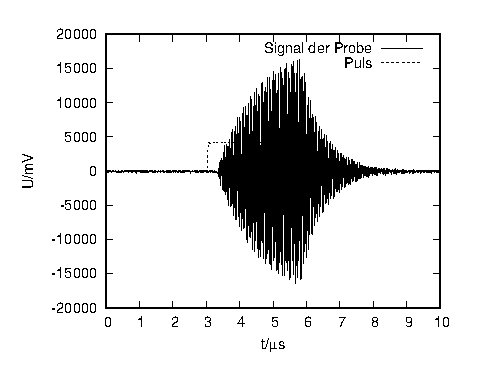
\includegraphics[width=0.75 \linewidth]{data/p402_443_data/pickup_probe/pickup.eps}
  \caption{Signal der Pickup-Probe}
  \label{fig:pickup}
\end{figure}

\subsection{Rabi-Oszillationen}
Die aufgenommene Amplitude des Antwortsignals (Envelope-Signal) als auch das In-Phase Antwortsignal werden gegen die Zeit aufgetragen (siehe Abbildung \ref{fig:rabi}). Der Fehler auf die Spannungswerte wird aus dem Untergrundrauschen gewonnen. An die Amplitude des Antwortsignals wird die Funktion
\begin{align*}
  U(t)=U_b+U_o|\sin(\omega t+\delta)|
\end{align*}
angepasst. An das In-Phase Signal wird die Funktion
\begin{align*}
  U(t)=U_b+U_o\sin(\omega t+\delta)
\end{align*}
angepasst. Die jeweiligen Parameter sind in Tabelle \ref{tab:rabi} zu sehen. Bis auf zwei Datenpunkte des Envelope-Signals wird der Verlauf gut von den Regressionskurven beschrieben. An den ermittelten Werten für $\omega$ und $\delta$ ist auch zu erkennen, dass die Signale, wie erwartet, Phasengleich sind. Die unterschiedlichen Werte für $U_0$ kommen durch die im Gerät passierende Umrechnung von Envelope Signal in In-Phase Signal zustande.

\begin{table}[h]
  \centering
  \begin{tabular}{c c c c c}
    \toprule
    Signal & $U_b/\mathrm{V}$ & $U_0/\mathrm{V}$ & $\omega \cdot \mu\mathrm{s}$ & $\delta$ \\
    \midrule
    Amplitude & $0,6 \pm 0,3$ & $8 \pm 0,3$ & $0,638 \pm 0,005$ & $-0,01 \pm 0,04$ \\
    In-Phase & $0,061 \pm 0,009$ & $1,3 \pm 0,01$& $0,635 \pm 0,003$ & $0,01 \pm 0,02$ \\
    \bottomrule
  \end{tabular}
  \caption{Regressionsparameter für Rabi-Oszillationen}
  \label{tab:rabi}
\end{table}

\begin{figure}[h]
  \centering
  \includegraphics[width=0.75 \linewidth]{data/p402_443_data/rabi_f_1/rabi_1.eps}
  \caption{Rabi-Oszillationen mit Regressionskurven}
  \label{fig:rabi}
\end{figure}

\newpage

\subsection{Vermessung der Spektralinien}
\label{subsec:auswertung_spektrallinien}
\subsubsection{Reflexionsgitter}
Um die Wellenlänge der Emissionslinien zu bestimmen, wird ein Reflexionsgitter verwendet. Untersucht wird dabei die Lage der Interferenzmaxima des reflektierten Lichtes. Eine wichtige Größe, die das Gitter charakterisiert, ist dabei die Gitterkonstante $g$, die die Periode des Gitters angibt. Mit Hilfe von Abbildung \ref{Gangunterschied} lässt sich leicht der Gangunterschied $s$ zweier benachbarter Strahlen berechnen. Werden die Winkel in mathematisch positiver Richtung zum Lot gemessen erhält man
\begin{align*}
  s=g \cdot (\sin(\alpha)+\sin(\beta)).
\end{align*} 
Für Licht der Wellenlänge $\lambda$ gilt bei den Interferenzmaxima also (mit $n \in \mathbb{Z}$)
\begin{align}
  g \cdot (\sin(\alpha)+\sin(\beta)) = n\lambda.
  \label{equ:gitter}
\end{align}
\begin{figure}[h]
  \centering
  \begin{tikzpicture}[scale=1.5]
    \draw (0,0)--(1,0);
    \draw [thick, dash dot] (0.5,0)--(0.5,3);
    \draw (-2,3)--(0.5,0);
    \draw [->] (0.5,0)--(-0.5,3);
    \draw (0.5,2.8) arc (90:108.5:2.8);
    \draw (0.5,2) arc (90:130:2);
    \draw (0.1,2.3) node {$\beta$};
    \draw (-0.3,1.5) node {$\alpha$};
    \draw (5,0)--(6,0);
    \draw [thick, dash dot] (5.5,0)--(5.5,3);
    \draw (5.5-2.5,3)--(5.5-2.5*0.82,3*0.82);
    \draw [line width=0.5mm] (5.5-2.5*0.82,3*0.82)--(5.5,0);
    \draw [line width=0.5mm] (5.5,0)--(5.5-0.5,0.5*3);
    \draw [->] (5.5-0.5,0.5*3)--(4.5,3);
    \draw (5.5,2.8) arc (90:108.5:2.8);
    \draw (5.5,2) arc (90:130:2);
    \draw (5.1,2.3) node {$\beta$};
    \draw (4.7,1.6) node {$\alpha$};
    \draw [dash dot](0.5,0)--(0.5+2.4*6/5,2.4);
    \draw [dash dot](0.5,0)--(0.5+1.5*3,1.5);
    \draw [<->] (0.5,-0.5)--(5.5,-0.5);
    \draw (3,-0.7) node {$g$};
    \draw (0.5+2.2*6/5,2.2) arc (220:325:0.3);
    \draw (3.4,2.25) node {$.$};
    \draw (0.5+1.4*3,1.4) arc (200:290:0.3);
    \draw (4.9,1.35) node {$.$};
  \end{tikzpicture}
  \caption{Gangunterschied (fett eingezeichnet) für benachbarte Strahlen}
  \label{Gangunterschied}
\end{figure}

Im Experiment kann man allerdings die Winkel $\alpha$ und $\beta$ nicht direkt messen, sondern man misst die Winkel $\omega\ind{G}$ und $\omega\ind{B}$ (siehe Abb. \ref{aufbau2}). Daraus ergibt sich:
\begin{align}
\alpha = \omega\ind{G}, \beta = \omega\ind{G}+\omega\ind{B}-180^\circ.
\label{equ:angle}
\end{align}
Während des gesamten Versuches war $\omega\ind{B}=150^\circ \pm 0,5^\circ$.

\subsubsection{Bestimmung der Gitterkonstanten}
\begin{figure}[h]
  \centering
  \includegraphics[width=0.75\linewidth]{data/Balmer/out_hg_raw.png}
  \caption{Gemessene Winkel $\omega\ind{G}$ der Spektralinien der Hg-Lampe}
  \label{fig:hg_raw}
\end{figure}

Da man die beiden gelben Linien nicht unterscheiden konnte, haben wir für die Wellenlänge der gelben Linie (roter Punkt, siehe Abb. \ref{fig:hg_raw}) den Mittelwert beider Linien angesetzt: $\lambda = \si{(578,013 \pm 1,053) \nano \metre}$. Nach Gl. \ref{equ:angle} werden $\alpha$ und $\beta$ berechnet. In Abb. \ref{fig:hg} ist $\lambda$ über $\sin{\alpha} + \sin{\beta}$ aufgetragen \footnote{$\Delta \sin{\alpha} = |\cos{\alpha} \cdot \Delta \alpha|$, $\Delta beta$ analog}. Zusätzlich ist in das Diagramm ein linearer Fit $y = a\cdot x + b$ an diese Daten eingezeichnet.
\begin{figure}[h]
  \centering
  \includegraphics[width=0.75\linewidth]{data/Balmer/out_hg.png}
  \caption{Bestimmung der Gitterkonstante}
  \label{fig:hg}
\end{figure}

Der Fit ergibt $a = \si{(653 \pm 36) \nano\metre}, b = \si{(-249 \pm 43) \nano\metre}$. Die Gitterkonstante beträgt also $g = a = \si{(653 \pm 36) \nano\metre}$. Nach Gl. \ref{equ:gitter} sollte $b \approx 0$ sein. Dies könnte aufgrund eines kleinen systematischen Fehlers auftreten (z.B. ein kleiner Offset bei der Winkelmessung). Extrapoliert man die Funktion bis $x = 0$, so liegt $\lambda = 0$ im Fehlerbereich. Führt man einen Fit ohne Achsenabschnitt $y = a\cdot x$ durch, so ergibt sich: $\si{(444 \pm 11) \nano\metre}$. Allerdings passt sich ein Fit mit Achsenabschnitt besser den Daten an, weswegen wir  entschieden haben, mit der Relation
\begin{align}
\lambda = g (\sin{\alpha} + \sin{\beta}) + b
\label{equ:gitter_neu}
\end{align}
weiterzuarbeiten.

\subsubsection{Untersuchung der Balmerlinien mit Okular}

\begin{table}
\centering
\caption{Messung mit dem Okular}
\begin{tabular}{c>{$}c<{$}>{$}c<{$}}
\toprule
Linie & \omega\ind{G}/^\circ & d/\si{\milli \metre}\\
\midrule
H$_\alpha$ & 60,5 \pm 0,5 &0,1\pm 0,05\\
H$_\beta$ & 53	\pm 0,5 &0,3\pm 0,05\\ 
H$_\gamma$ & 48,5 \pm 0,5\\
H$_\delta$ & 48\pm 0,5\\
H$_\epsilon$ & 46\pm 0,5\\
\bottomrule
\end{tabular}
\label{tab:okular}
\end{table}

In Tab. \ref{tab:okular} sind die gemessenen Winkel und die Aufspaltung der einzelnen Linien eingetragen. Die Aufspaltung konnte nur für die H$_\alpha$- und H$_\beta$-Linie bestimmt werden. Die Wellenlängen der Linien wurden über Gl. \ref{equ:angle} und Gl. \ref{equ:gitter_neu} berechnet. Um die Isotopieaufspaltung $\delta \lambda$ zu berechnen, linearisiert man Gl. \ref{equ:gitter_neu}: $\delta \lambda = g\cos{\beta} \delta\beta$. $\delta \beta$ ergibt sich aufgrund des nahezu parallelen Lichtes durch: $\delta\beta = \arctan{\frac{d}{f}} \overset{d \ll f}{=} \frac{d}{f}$, wobei $f$ die Brennweite des Objektives ist. Da wir keine Angabe über den Fehler von $f$ haben, haben wir den Fehler auf \si{10\milli \metre} geschätzt: $f = \si{(300\pm 10)\milli \metre}$.\\

In \ref{tab:okular_res} sind die berechneten Wellenlängen, die Isotopieaufspaltung sowie die theoretisch Werte\cite{wiki_balmer} angeben. Die wirklichen Wellenlängen liegen alle im Fehlerbereich der berechneten Werte.

\begin{table}
\centering
\caption{Ergebnisse der Messung mit dem Okular}
\begin{tabular}{c>{$}c<{$}>{$}c<{$}>{$}c<{$}}
\toprule
Linie & \lambda/\si{\nano\metre} & \lambda/\si{\nano\metre}\text{(Literatur \cite{wiki_balmer})} & \delta\lambda/\si{\nano \metre}\\
\midrule
H$_\alpha$ & 651\pm 56 & 656,278 & 0,19\pm 0,09\\
H$_\beta$ & 527 \pm	53 & 486,132 & 0,6\pm 0,1\\ 
H$_\gamma$ & 447 \pm 50 & 434,045\\
H$_\delta$ & 438 \pm 50 & 410,1735\\
H$_\epsilon$ & 400 \pm 49 & 397,0074\\
\bottomrule
\end{tabular}
\label{tab:okular}
\end{table}

\subsubsection{Untersuchung der Balmerlinien mit CCD-Kamera}
Die Programm berechnet eigenständig aus der Pixelkoordinate den dazugehörigen Winkel $\gamma$. Da wir keine Angaben zu den Fehlern der Kamera haben (sowohl für $\gamma$, als auch für die Intensität $I$), sind keine Fehler in den Diagrammen eingezeichnet. Für das weitere Vorgehen ist dies nicht relevant, da, wenn der Fehler für alle Werte gleich ist, das Ergebnis des Fitalgorithmus nicht beeinflusst wird. 

\begin{figure}[h]
  \centering
  \includegraphics[width=0.75\linewidth]{data/Balmer/out_red_raw.png}
  \caption{Intensitätsverteilung der H$_\alpha$-Linie}
  \label{fig:red_raw}
\end{figure}
\begin{figure}[h]
  \centering
  \includegraphics[width=0.75\linewidth]{data/Balmer/out_lightblue_raw.png}
  \caption{Intensitätsverteilung der H$_\beta$-Linie}
  \label{fig:lightblue_raw}
\end{figure}
\begin{figure}[h]
  \centering
  \includegraphics[width=0.75\linewidth]{data/Balmer/out_blue_raw.png}
  \caption{Intensitätsverteilung der (v.l.n.r.) H$_\gamma$-,H$_\delta$- und H$_\epsilon$-Linie}
  \label{fig:blue_raw}
\end{figure}

In den Abbildungen \ref{fig:red_raw}-\ref{fig:blue_raw} sind die von der Kamera gemittelten Werte aufgetragen. Nun wird um jede Linie ein möglichst kleiner Ausschnitt genommen (siehe Abb. \ref{fig:red} - \ref{fig:blue2}). Kann man in diesem Ausschnitt 2 getrennte Linien erkennen (H$_\alpha$, H$_\beta$, H$_\delta$), wird an ihn die Summe zweier Gaussfunktionen angefittet:
\begin{align*}
I(\gamma) = a_1\exp{-\frac{(\gamma-b_1)^2}{2s_1^2}} + a_2\exp{-\frac{(\gamma-b_2)^2}{2s_2^2}} + d
\end{align*}
Leider war die Intensität der H$_\gamma$- und H$_\epsilon$-Linie nicht groß genug, um zwei Linien erkennen zu können. Deswegen wird nur eine Gaussfunktion an den Ausschnitt gefittet:
\begin{align*}
I(\gamma) = a_1\exp{-\frac{(\gamma-b_1)^2}{2s_1^2}} + d
\end{align*}
Das d haben wir aufgrund eines nicht vernachlässigbaren Untergrundes hinzugefügt. Die Ergebnisse der Fits sind in Tab. \ref{tab:ccd_fit} dargestellt.

\begin{figure}[h]
  \centering
  \includegraphics[width=0.75\linewidth]{data/Balmer/out_red.png}
  \caption{Fit an die H$_\alpha$-Linie}
  \label{fig:red}
\end{figure}
\begin{figure}[h]
  \centering
  \includegraphics[width=0.75\linewidth]{data/Balmer/out_lightblue.png}
  \caption{Fit an die H$_\beta$-Linie}
  \label{fig:lightblu}
\end{figure}
\begin{figure}[h]
  \centering
  \includegraphics[width=0.75\linewidth]{data/Balmer/out_blue0.png}
  \caption{Fit an die H$_\gamma$-Linie}
  \label{fig:blue0}
\end{figure}
\begin{figure}[h]
  \centering
  \includegraphics[width=0.75\linewidth]{data/Balmer/out_blue1.png}
  \caption{Fit an die H$_\delta$-Linie}
  \label{fig:blue1}
\end{figure}
\begin{figure}[h]
  \centering
  \includegraphics[width=0.75\linewidth]{data/Balmer/out_blue2.png}
  \caption{Fit an die H$_\epsilon$-Linie}
  \label{fig:blue2}
\end{figure}

\begin{table}[h]
\centering
\caption{Ergebnisse der Fits an die Linien}
\begin{tabular}{>{$}c<{$}>{$}c<{$}>{$}c<{$}>{$}c<{$}>{$}c<{$}>{$}c<{$}>{$}c<{$}}
\toprule
& H_\alpha & H_\beta & H_\gamma & H_\delta & H_\epsilon\\
\midrule
a_1 & 85 \pm 1 	& 40,4 \pm 0,5 	& 3,01 \pm 0,03	& 26,3 \pm 0,1 	& 2,79\pm 0,02\\
a_2 & 47 \pm 2 	& 3,8\pm 0,6 	& 	& 1,7 \pm 0,1 \\ 		
b_1 & -0,3357 \pm 5\cdot 10^{-4} & 0,30481\pm 8\cdot 10^{-5} & -1,5352\pm 2\cdot 10^{-4} & -1,1607 \pm 1\cdot 10^{-4} & 2,0022 \pm 2\cdot 10^{-4}\\
b_2 & -0,3024 \pm 5 \cdot 10^{-4}	& 0,3244\pm 7\cdot 10^{-4} 	& 	& -1,258 \pm 1\cdot 10^{-3} 	&\\
s_1 & 0,0164 \pm 5\cdot 10^{-4} & 0,00508\pm 8\cdot 10^{-5} 	& 0,0223\pm 3\cdot 10^{-4} & 0,0243 \pm 1\cdot 10^{-4} 	&  0,0276\pm 3\cdot 10^{-4}\\
s_2 & 0,0078 \pm 5\cdot 10^{-4} 	& 0,0037\pm 7\cdot 10^{-4} & & 0,024\pm 2\cdot 10^{-3}	\\
d & 11,7 \pm 0,6	& 11,3 \pm 0,2	& 6,36\pm 0,02 & 6,91  \pm 0,04 & 14,49\pm 0,01\\
\bottomrule
\end{tabular}
\label{tab:okular}
\end{table}
\section{Fazit}
Wir haben Bilder von der Oberfläche von Graphit, Gold und TaS$_2$ in der Größenordung von 100nm aufgenommen. Zusätzlich war es möglich ein Bild der Graphitoberfläche mit atomarer Auflösung zu erstellen. Mithilfe dieser Aufnahme konnten wir nach Entzerrung des Bildes bestätigen, dass die Bindungswinkel der Graphitstruktur $120^\circ \pm 3^\circ$ beträgt, es sich also um eine Struktur aus regelmäßigen Sechsecken handelt. Der Atomabstand wurde zu $a = 0,179\si{\nano\metre} \pm 0,002\si{\nano\metre}$ bestimmt. Dies weicht deutlich vom Literaturwert $l=0,142$ nm ab. Gründe für diese Abweichung wurden erläutert.




\begin{table}
\centering
\caption{Fitparameter und berechnete Gangunterschiede}
\label{tab:werte}
\begin{tabular}{S[round-mode=places,round-precision=1]S[round-mode=places,round-precision=0]S[round-mode=places,round-precision=2]S[round-mode=places,round-precision=2]S[round-mode=places,round-precision=2]S[round-mode=places,round-precision=2]S[round-mode=places,round-precision=2]S[round-mode=places,round-precision=2]S[round-mode=places,round-precision=9]S[round-mode=places,round-precision=2]}
{$I/\si{\ampere}$}	&	{n}	&	{$a/\%$}	&	{$\Delta a/\%$}	&	{$b$}	&	{$\Delta b$}	&	{$s$}	&	{$\Delta s$}	&	{$g/\si{\si{m}}$}	&	{$\Delta g/\si{\meter}$}\\
\toprule
6	&	1	&	28,5016	&	0,849783	&	829,358	&	0,492301	&	12,95453556	&	0,704329829	&	0,011655094	&	4,58358E-09\\
6	&	2	&	21,1055	&	1,16465	&	849,878	&	0,187483	&	4,834382153	&	0,247274946	&	0,011655275	&	1,56152E-09\\
6	&	3	&	38,5883	&	0,293881	&	871,119	&	0,534864	&	19,33226282	&	0,704277171	&	0,011655441	&	3,91131E-09\\
6	&	4	&	21,6083	&	0,782926	&	921,91	&	0,35641	&	13,000314	&	0,459584163	&	0,011655751	&	1,74039E-09\\
6	&	5	&	51,5363	&	0,462747	&	979,654	&	0,684621	&	32,27108592	&	0,92221909	&	0,011655953	&	1,45215E-09\\
6	&	6	&	51,7062	&	0,356072	&	1065,99	&	0,729291	&	34,32797346	&	0,989290033	&	0,011655958	&	1,46471E-09\\
6	&	7	&	20,074	&	0,738264	&	1125,08	&	0,323965	&	12,08075329	&	0,429837517	&	0,011655756	&	1,56631E-09\\
6	&	8	&	34,5089	&	0,302	&	1174,27	&	0,616481	&	18,09819824	&	0,699844561	&	0,01165546	&	4,43115E-09\\
6	&	9	&	27,9089	&	1,64872	&	1195,93	&	0,22516	&	6,153073153	&	0,272019088	&	0,011655293	&	1,85171E-09\\
6	&	10	&	28,7849	&	0,674773	&	1216,72	&	0,378693	&	11,12059499	&	0,480340739	&	0,011655112	&	3,49101E-09\\
\midrule
6,3	&	1	&	31,387	&	0,903664	&	829,069	&	0,574861	&	14,16337527	&	0,755105684	&	0,011655091	&	5,36021E-09\\
6,3	&	2	&	21,2711	&	1,1059	&	850,298	&	0,178191	&	4,835910933	&	0,238872606	&	0,011655278	&	1,48054E-09\\
6,3	&	3	&	41,3403	&	0,327233	&	871,999	&	0,567802	&	19,46178439	&	0,77409482	&	0,011655447	&	4,12827E-09\\
6,3	&	4	&	24,7343	&	0,851412	&	921,952	&	0,358973	&	13,3563497	&	0,448894599	&	0,011655751	&	1,75218E-09\\
6,3	&	5	&	54,4236	&	0,611898	&	979,675	&	0,729286	&	31,71724317	&	0,915764245	&	0,011655953	&	1,54615E-09\\
6,3	&	6	&	55,7872	&	0,389607	&	1064,36	&	0,779025	&	34,96972101	&	1,041599763	&	0,011655961	&	1,50386E-09\\
6,3	&	7	&	22,6951	&	0,813742	&	1125,32	&	0,340425	&	12,76683544	&	0,45117248	&	0,011655754	&	1,64979E-09\\
6,3	&	8	&	37,0904	&	0,308758	&	1172,36	&	0,518518	&	17,17846766	&	0,687165036	&	0,011655474	&	3,67963E-09\\
6,3	&	9	&	32,5284	&	1,88681	&	1195,29	&	0,219756	&	6,567635617	&	0,265695037	&	0,011655298	&	1,80054E-09\\
6,3	&	10	&	32,4417	&	0,500637	&	1216,77	&	0,373865	&	11,63001821	&	0,50501014	&	0,011655111	&	3,4474E-09\\
\midrule
6,6	&	1	&	32,9667	&	0,837135	&	828,568	&	0,523639	&	14,07784857	&	0,754080552	&	0,011655087	&	4,89515E-09\\
6,6	&	2	&	22,9343	&	1,25389	&	850,404	&	0,187006	&	5,14689011	&	0,251028949	&	0,011655279	&	1,55284E-09\\
6,6	&	3	&	41,9592	&	0,314762	&	872,619	&	0,520596	&	19,21310297	&	0,800620839	&	0,011655452	&	3,76961E-09\\
6,6	&	4	&	25,9236	&	0,8841	&	921,446	&	0,377889	&	13,44586822	&	0,459544245	&	0,011655748	&	1,85366E-09\\
6,6	&	5	&	55,8408	&	0,583553	&	980,444	&	0,747632	&	32,03174704	&	0,933795347	&	0,011655955	&	1,55755E-09\\
6,6	&	6	&	56,2759	&	0,439048	&	1064,42	&	0,787264	&	34,0842181	&	1,018642594	&	0,011655961	&	1,52203E-09\\
6,6	&	7	&	24,7069	&	0,822702	&	1125,89	&	0,36283	&	13,15947691	&	0,46998241	&	0,011655752	&	1,76827E-09\\
6,6	&	8	&	37,4038	&	0,308416	&	1171,1	&	0,456895	&	16,40779306	&	0,702014578	&	0,011655483	&	3,21479E-09\\
6,6	&	9	&	36,0039	&	1,99397	&	1195,1	&	0,222528	&	6,849007436	&	0,265326432	&	0,0116553	&	1,82123E-09\\
6,6	&	10	&	33,6566	&	0,401879	&	1217,24	&	0,362931	&	11,62730038	&	0,525996881	&	0,011655107	&	3,35474E-09\\
\midrule
6,9	&	1	&	34,9489	&	0,790265	&	828,234	&	0,483548	&	14,035977	&	0,747562007	&	0,011655083	&	4,52809E-09\\
6,9	&	2	&	24,699	&	1,40797	&	850,528	&	0,193453	&	5,405551064	&	0,259990143	&	0,01165528	&	1,60522E-09\\
6,9	&	3	&	43,2783	&	0,312716	&	873,167	&	0,47974	&	18,9233993	&	0,820184117	&	0,011655456	&	3,4612E-09\\
6,9	&	4	&	27,6339	&	0,926272	&	921,057	&	0,394872	&	13,61607231	&	0,46921802	&	0,011655747	&	1,94431E-09\\
6,9	&	5	&	57,3809	&	0,640938	&	980,383	&	0,759464	&	31,74586532	&	0,928036945	&	0,011655955	&	1,58441E-09\\
6,9	&	6	&	58,0811	&	0,452129	&	1063,81	&	0,803813	&	34,23327408	&	1,036121637	&	0,011655962	&	1,53057E-09\\
6,9	&	7	&	26,2347	&	0,853151	&	1126,35	&	0,382387	&	13,43644074	&	0,491045591	&	0,011655749	&	1,87199E-09\\
6,9	&	8	&	38,5257	&	0,315227	&	1170,26	&	0,415746	&	15,8111445	&	0,698357398	&	0,011655488	&	2,90855E-09\\
6,9	&	9	&	38,9209	&	2,09986	&	1194,88	&	0,225543	&	7,062110769	&	0,267110008	&	0,011655302	&	1,84353E-09\\
6,9	&	10	&	35,0754	&	0,366594	&	1217,52	&	0,36928	&	11,77126042	&	0,556452712	&	0,011655104	&	3,41837E-09\\
\midrule
7,2	&	1	&	38,302	&	0,708121	&	828,184	&	0,56175	&	15,21712883	&	0,8582142	&	0,011655083	&	5,26174E-09\\
7,2	&	2	&	26,0178	&	1,5707	&	850,905	&	0,200594	&	5,652007264	&	0,275845282	&	0,011655283	&	1,66086E-09\\
7,2	&	3	&	45,8882	&	0,375954	&	874,16	&	0,486584	&	18,29218334	&	0,854689514	&	0,011655463	&	3,48746E-09\\
7,2	&	4	&	30,1839	&	1,03816	&	920,77	&	0,427836	&	13,93286934	&	0,499785961	&	0,011655745	&	2,1125E-09\\
7,2	&	5	&	61,1654	&	0,712664	&	981,081	&	0,817231	&	32,09145436	&	0,987837693	&	0,011655956	&	1,67764E-09\\
7,2	&	6	&	61,7975	&	0,55241	&	1063,86	&	0,849066	&	33,86432869	&	1,072183841	&	0,011655962	&	1,61877E-09\\
7,2	&	7	&	29,2271	&	0,917013	&	1127,07	&	0,396656	&	14,04514968	&	0,527519715	&	0,011655746	&	1,95551E-09\\
7,2	&	8	&	41,2495	&	0,32468	&	1169,45	&	0,356187	&	14,78983503	&	0,648990569	&	0,011655494	&	2,47808E-09\\
7,2	&	9	&	44	&	2,23267	&	1194,55	&	0,22516	&	7,294510694	&	0,264115299	&	0,011655304	&	1,83685E-09\\
7,2	&	10	&	37,9037	&	0,358754	&	1217,76	&	0,387836	&	12,05111196	&	0,600131633	&	0,011655102	&	3,59459E-09\\
\bottomrule
\end{tabular}
\end{table}

\begin{table}\ContinuedFloat
\caption{Fitparameter und berechnete Gangunterschiede}  
\centering
\begin{tabular}{S[round-mode=places,round-precision=1]S[round-mode=places,round-precision=0]S[round-mode=places,round-precision=2]S[round-mode=places,round-precision=2]S[round-mode=places,round-precision=2]S[round-mode=places,round-precision=2]S[round-mode=places,round-precision=2]S[round-mode=places,round-precision=2]S[round-mode=places,round-precision=9]S[round-mode=places,round-precision=2]}
{$I/\si{\ampere}$}	&	{n}	&	{$a/\%$}	&	{$\Delta a/\%$}	&	{$b$}	&	{$\Delta b$}	&	{$s$}	&	{$\Delta s$}	&	{$g/\si{\si{m}}$}	&	{$\Delta g/\si{\meter}$}\\
\toprule
7,5	&	1	&	41,2826	&	0,680767	&	828,008	&	0,545552	&	15,36465603	&	0,896501626	&	0,011655081	&	5,11461E-09\\
7,5	&	2	&	28,3209	&	1,87001	&	851,149	&	0,214097	&	5,950348533	&	0,296231553	&	0,011655285	&	1,77016E-09\\
7,5	&	3	&	48,3495	&	0,395294	&	874,763	&	0,462635	&	17,95763548	&	0,892773104	&	0,011655467	&	3,30247E-09\\
7,5	&	4	&	32,5046	&	1,17099	&	920,533	&	0,467175	&	14,18902479	&	0,536565842	&	0,011655744	&	2,31204E-09\\
7,5	&	5	&	64,4808	&	0,808608	&	981,499	&	0,884953	&	32,25817623	&	1,056649745	&	0,011655957	&	1,79897E-09\\
7,5	&	6	&	65,0908	&	0,661405	&	1063,61	&	0,908542	&	33,63229397	&	1,130311425	&	0,011655962	&	1,72129E-09\\
7,5	&	7	&	31,8436	&	0,997837	&	1127,42	&	0,416964	&	14,53962483	&	0,568136832	&	0,011655744	&	2,06261E-09\\
7,5	&	8	&	43,5807	&	0,342122	&	1168,81	&	0,324144	&	14,21195648	&	0,623659546	&	0,011655498	&	2,24522E-09\\
7,5	&	9	&	46,1835	&	2,43014	&	1194,05	&	0,220252	&	7,360375599	&	0,266090821	&	0,011655308	&	1,79154E-09\\
7,5	&	10	&	40,1569	&	0,368355	&	1217,84	&	0,438522	&	13,16780026	&	0,679554263	&	0,011655101	&	4,06605E-09\\
\midrule
7,8	&	1	&	44,3432	&	0,594238	&	827,832	&	0,504399	&	15,39828917	&	0,923178824	&	0,01165508	&	4,73305E-09\\
7,8	&	2	&	31,74	&	2,31542	&	851,42	&	0,229708	&	6,366235939	&	0,318516059	&	0,011655288	&	1,89626E-09\\
7,8	&	3	&	50,5466	&	0,400049	&	875,54	&	0,417655	&	17,35699511	&	0,897130124	&	0,011655473	&	2,96586E-09\\
7,8	&	4	&	35,0287	&	1,26995	&	920,192	&	0,501846	&	14,45511731	&	0,570512385	&	0,011655742	&	2,49181E-09\\
7,8	&	5	&	67,6685	&	0,890704	&	981,874	&	0,929589	&	32,3045492	&	1,100313379	&	0,011655958	&	1,87304E-09\\
7,8	&	6	&	67,8515	&	0,754651	&	1063,39	&	0,950983	&	33,42013338	&	1,174212869	&	0,011655963	&	1,7917E-09\\
7,8	&	7	&	34,3721	&	1,05001	&	1127,94	&	0,428857	&	15,04097949	&	0,602698284	&	0,011655742	&	2,13211E-09\\
7,8	&	8	&	45,4338	&	0,39049	&	1168,22	&	0,311988	&	13,52426062	&	0,589696866	&	0,011655503	&	2,15222E-09\\
7,8	&	9	&	50,1631	&	2,51562	&	1193,75	&	0,224523	&	7,567567652	&	0,268998899	&	0,011655311	&	1,82306E-09\\
7,8	&	10	&	42,1569	&	0,387785	&	1218,21	&	0,449665	&	13,40951724	&	0,73323225	&	0,011655098	&	4,17733E-09\\
\midrule
8,1	&	1	&	46,3447	&	0,509655	&	827,661	&	0,470755	&	15,19937801	&	0,932351499	&	0,011655078	&	4,4212E-09\\
8,1	&	2	&	35,3236	&	2,86218	&	851,697	&	0,251792	&	6,830279891	&	0,345449752	&	0,01165529	&	2,07523E-09\\
8,1	&	3	&	51,7416	&	0,394986	&	876,184	&	0,387468	&	16,57731769	&	0,889511708	&	0,011655477	&	2,73956E-09\\
8,1	&	4	&	36,7468	&	1,34075	&	919,753	&	0,538484	&	14,81030369	&	0,620650399	&	0,01165574	&	2,68504E-09\\
8,1	&	5	&	69,1708	&	0,985701	&	982,084	&	0,988512	&	32,35211122	&	1,166883221	&	0,011655958	&	1,98183E-09\\
8,1	&	6	&	69,563	&	0,849667	&	1063,12	&	1,01673	&	33,39643731	&	1,224552172	&	0,011655963	&	1,90244E-09\\
8,1	&	7	&	35,9677	&	1,10244	&	1128,05	&	0,441632	&	15,18468474	&	0,621584653	&	0,011655741	&	2,19794E-09\\
8,1	&	8	&	46,5887	&	0,430544	&	1167,8	&	0,3148	&	13,33639064	&	0,590675284	&	0,011655505	&	2,16529E-09\\
8,1	&	9	&	52,3572	&	2,55288	&	1193,54	&	0,226993	&	7,667558308	&	0,271315849	&	0,011655313	&	1,84083E-09\\
8,1	&	10	&	43,5912	&	0,402399	&	1218,43	&	0,442168	&	13,50030974	&	0,750254358	&	0,011655096	&	4,11233E-09\\
\midrule
8,4	&	1	&	47,8795	&	0,478622	&	827,212	&	0,443963	&	14,97031592	&	0,935188234	&	0,011655074	&	4,17911E-09\\
8,4	&	2	&	38,5479	&	3,33642	&	851,976	&	0,273361	&	7,266720884	&	0,36839503	&	0,011655292	&	2,24934E-09\\
8,4	&	3	&	52,2805	&	0,407569	&	876,843	&	0,39482	&	16,19401877	&	0,936861398	&	0,011655482	&	2,77909E-09\\
8,4	&	4	&	38,2307	&	1,42404	&	919,486	&	0,584402	&	15,00887513	&	0,656890111	&	0,011655739	&	2,92146E-09\\
8,4	&	5	&	70,5172	&	1,01235	&	982,67	&	1,02937	&	32,54643605	&	1,211345218	&	0,011655959	&	2,0349E-09\\
8,4	&	6	&	70,6209	&	0,953517	&	1063,09	&	1,04716	&	33,00141774	&	1,232187575	&	0,011655963	&	1,95787E-09\\
8,4	&	7	&	37,8303	&	1,10571	&	1128,39	&	0,446596	&	15,51252295	&	0,633863298	&	0,011655739	&	2,22991E-09\\
8,4	&	8	&	47,174	&	0,501739	&	1167,38	&	0,313046	&	12,96345343	&	0,572712978	&	0,011655508	&	2,14694E-09\\
8,4	&	9	&	54,8166	&	2,47804	&	1193,32	&	0,226677	&	7,811993973	&	0,26954926	&	0,011655314	&	1,83588E-09\\
8,4	&	10	&	44,7114	&	0,410544	&	1218,82	&	0,422527	&	13,55143892	&	0,759990983	&	0,011655092	&	3,93755E-09\\
\midrule
8,5	&	1	&	48,6808	&	0,464019	&	826,953	&	0,435262	&	14,7116125	&	0,926907347	&	0,011655071	&	4,1026E-09\\
8,5	&	2	&	40,8743	&	3,56628	&	852,015	&	0,283909	&	7,482440128	&	0,376036378	&	0,011655293	&	2,33561E-09\\
8,5	&	3	&	52,6448	&	0,439247	&	877,097	&	0,401461	&	15,89369858	&	0,944513788	&	0,011655484	&	2,82096E-09\\
8,5	&	4	&	39,2747	&	1,44171	&	919,239	&	0,599965	&	15,14935295	&	0,675250749	&	0,011655738	&	3,00635E-09\\
8,5	&	5	&	70,8515	&	1,10113	&	982,363	&	1,04293	&	32,23651852	&	1,212330431	&	0,011655959	&	2,07702E-09\\
8,5	&	6	&	71,5573	&	0,941165	&	1062,65	&	1,07351	&	33,35193284	&	1,270899662	&	0,011655964	&	1,98454E-09\\
8,5	&	7	&	38,3556	&	1,13846	&	1128,63	&	0,458443	&	15,61342238	&	0,649582546	&	0,011655738	&	2,29433E-09\\
8,5	&	8	&	47,4932	&	0,545388	&	1167,17	&	0,316284	&	12,79885487	&	0,571046608	&	0,01165551	&	2,16597E-09\\
8,5	&	9	&	55,9936	&	2,47571	&	1193,21	&	0,22898	&	7,893087219	&	0,272269637	&	0,011655315	&	1,85333E-09\\
8,5	&	10	&	45,3822	&	0,417133	&	1219	&	0,417693	&	13,59874614	&	0,77311895	&	0,011655091	&	3,8961E-09\\
\bottomrule
\end{tabular}
\end{table}


  \begin{table}[h]
    \centering
    \begin{tabular}{c | r p{0.05cm} l r p{0.05cm} l r p{0.05cm} l r p{0.05cm} l}
      \toprule
       $U_\mathrm{G}/$V & & 1 & & & 2 & & & 3 & & & 4 &\\  
      \midrule
      $U_0/$V &              -1,1         &$\pm$ & 0,1      &   -0,9        &$\pm$ & 0,1     & -0,7  & $\pm$ &  0,1  &  -0,062  & $\pm$  & 0,004 \\    
      $\alpha$ & 0,101         &$\pm$ & 0,006    &  0,052        &$\pm$ & 0,005    & 0,03  & $\pm$ & 0,005   &   0,0007 & $\pm$  & 0,002 \\
      $A_1$/V &              0,38         &$\pm$ & 0,06     &   0,45          &$\pm$ & 0,07    & 0,41  & $\pm$ &  0,09  &    &   &  \\ 
      $A_2$/V &              0,82         &$\pm$ & 0,03     &   0,63         &$\pm$ & 0,03    &  0,36 & $\pm$ & 0,04   &  0,039  & $\pm$  & 0,005 \\ 
      $A_3$/V &             1,85          &$\pm$ & 0,02     &   1,21          &$\pm$ & 0,03    & 0,58  & $\pm$ & 0,03   &  0,104  & $\pm$  & 0,005 \\ 
      $A_4$/V &              3,49          &$\pm$ & 0,04     &   2,09          &$\pm$ & 0,02    & 0,9  & $\pm$ &  0,02  &  0,208  & $\pm$  & 0,005 \\ 
      $A_5$/V &              41          &$\pm$ & 83       &   1,6          &$\pm$ & 0,6     & 0,2  & $\pm$ & 0,1   &    &  &  \\ 
      $\mu_1/$V &            11,38          &$\pm$ & 0,08     &   11,6            &$\pm$ & 0,1     & 11,4  & $\pm$ & 0,2   &    &   &  \\ 
      $\mu_2/$V &           16,29          &$\pm$ & 0,02     &  16,64          &$\pm$ & 0,04    &  17,01 & $\pm$ & 0,09   &  17  & $\pm$  & 0,1 \\ 
      $\mu_3/$V &            21,11           &$\pm$ & 0,01      &   21,34           &$\pm$ & 0,02     & 21,58  & $\pm$ & 0,02   &   21,88 & $\pm$  & 0,04 \\ 
      $\mu_4/$V &            26,01          &$\pm$ & 0,01    &   26,28          &$\pm$ & 0,01   & 26,47  & $\pm$ & 0,02   &  26,83  & $\pm$ & 0,02 \\ 
      $\mu_5/$V &            34          &$\pm$ & 2       &   30,5          &$\pm$ & 0,4     & 30,1  & $\pm$ &  0,3  &    &  &  \\ 
      $\sigma_1$/V &         1,4          &$\pm$ & 0,2      &   2,1          &$\pm$ & 0,2     & 2,8  & $\pm$ & 0,4   &    &   &  \\ 
      $\sigma_2$/V &         0,87         &$\pm$ & 0,04     &   1,08          &$\pm$ & 0,05    & 1,34  & $\pm$ &  0,09  &  0,8  & $\pm$  & 0,1 \\ 
      $\sigma_3$/V &         0,82         &$\pm$ & 0,01      &   0,94         &$\pm$ & 0,03    & 1,07  & $\pm$ & 0,06   &   0,79 & $\pm$  & 0,05 \\ 
      $\sigma_4$/V &        0,9          &$\pm$ & 0,01    &   0,89         &$\pm$ & 0,02    &  0,91 & $\pm$ &  0,02  &  0,86  & $\pm$  & 0,03 \\ 
      $\sigma_5$/V &         1,7          &$\pm$ & 0,5      &   0,6         &$\pm$ & 0,1     & 0,2  & $\pm$ & 0,1   &    &   &  \\ 
      \bottomrule
    \end{tabular}
    \caption{Parameter der Regressionskurven für Frank-Hertz-Versuch}
    \label{tab:fh_parameter_1}
  \end{table}

 \begin{table}[h]
    \centering
    \begin{tabular}{c | r p{0.05cm} l r p{0.05cm} l r p{0.05cm} l r p{0.05cm} l r p{0.05cm} l}
      \toprule
       $T/^\circ$C & & 159 & & & 168 & & & 173 & & & 175 & & & 181& \\  
      \midrule
      $U_0/$V &              -0,072         &$\pm$ & 0,005      &   -0,071        &$\pm$ & 0,002     & -0,072  & $\pm$ &  0,003  &  -0,068  & $\pm$  & 0,002 & -0,073 & $\pm$ & 0,002\\    
      $\alpha$& 0,0012         &$\pm$ & 0,0003    &  0,0009        &$\pm$ & 0,0001    & 0,0008  & $\pm$ & 0,0001   &   0,0005 & $\pm$  & 0,0001 & 0,0002 & $\pm$ & 0,0001\\
      $A_2$/V &              0,041         &$\pm$ & 0,005     &   0,029          &$\pm$ & 0,003    &   &  &   &    &   &  & & &\\ 
      $A_3$/V &              0,117         &$\pm$ & 0,006     &   0,065         &$\pm$ & 0,003    &  0,041 & $\pm$ & 0,003   &  0,021  & $\pm$  & 0,002 & 0,016 & $\pm$ & 0,002\\ 
      $A_4$/V &              0,237          &$\pm$ & 0,006     &   0,133          &$\pm$ & 0,003    & 0,095  & $\pm$ & 0,003   &  0,052  & $\pm$  & 0,002 & 0,029 & $\pm$ & 0,002\\ 
      $\mu_2/$V &            17,1          &$\pm$ & 0,1     &   17,16            &$\pm$ & 0,09     &   &  &    &   &   & & & &\\ 
      $\mu_3/$V &            21,91          &$\pm$ & 0,04     &   21,93          &$\pm$ & 0,04    &  21,99 & $\pm$ & 0,06   &  22,2  & $\pm$  & 0,1 & 22,27 & $\pm$ & 0,09\\ 
      $\mu_4/$V &            26,87,           &$\pm$ & 0,02      &   26,82           &$\pm$ & 0,02     & 26,83  & $\pm$ & 0,03   &   26,89 & $\pm$  & 0,04 & 27,23 & $\pm$ & 0,06\\ 
      $\sigma_2$/V &         0,8          &$\pm$ & 0,1      &   0,8          &$\pm$ & 0,1     &   &  &   &    &  &  &  & & \\ 
      $\sigma_3$/V &         0,87         &$\pm$ & 0,04     &   0,83          &$\pm$ & 0,04    & 0,76  & $\pm$ &  0,07  &  0,8  & $\pm$  & 0,1 & 0,8 & $\pm$ & 0,1\\ 
      $\sigma_4$/V &         0,82         &$\pm$ & 0,01      &   0,85         &$\pm$ & 0,02    & 0,83  & $\pm$ & 0,03   &   0,81 & $\pm$  & 0,05 & 1,02 & $\pm$ & 0,08\\ 
      \bottomrule
    \end{tabular}
    \caption{Parameter der Regressionskurven für Frank-Hertz-Versuch}
    \label{tab:fh_parameter_2}
  \end{table}

\begin{table}[h]
    \centering
    \begin{tabular}{c c c}
      \toprule
      $T/^\circ$C & $U_\mathrm{G}/$V & $\Delta \mu/$V\\
      \midrule
      165&1&$4,91\pm 0,09$\\
      &&$4,82\pm 0,03$\\
      &&$4,90 \pm 0,02$\\
      165&2&$5,1 \pm 0,1$\\
      &&$4,70 \pm 0,04$\\
      &&$4,93 \pm 0,02$\\
      165&3&$5,6 \pm 0,2$\\
      &&$4,51 \pm 0,09$\\
      &&$4,89 \pm 0,03$\\
      165&4&$4,8 \pm 0,1$\\
      &&$4,95 \pm 0,05$\\
      159&4&$4,8 \pm 0,1$\\
      &&$4,97 \pm 0,05$\\
      168&4&$4,8 \pm 0,1$\\
      &&$4,89 \pm 0,05$\\
      173&4&$4,85 \pm 0,07$\\
      175&4&$4,7 \pm 0,4$\\
      181&4&$5,00\pm 0,1$\\
      \bottomrule
    \end{tabular}
    \caption{Abstände von Spannungsmaxima in Frank-Hertz-Versuch}
    \label{tab:fh_dist}
  \end{table}


\newpage
\printbibliography

\end{document}
